\chapter{Numerical Studies}
Having discussed how the NSE were simplified, discretized, and implemented, in this section the implementation is tested and validated.
To this end, first the results of the unit tests from section \ref{sec:testing} are discussed by looking at the numerical errors made by the differential operators and integrators.
Thereafter the implementations of the non-hydrostatic NSE discussed in section \ref{sec:non_hydrostatic} are analyzed.

\section{Validation by Analyzing Numerical Errors}
In this section the results of the tests performed in section \ref{sec:testing} are discussed.

% analysis of errors
\subsection{Differential Operators}
To test the differential operators, the function $f(x)=\sin(20\pi (x-e))$ was used on the domain $[0;1]$.
The offset of $e$ was introduced in order to avoid random perfect results.
Without it, if, for example, the samples happen to be located at the maximums, minimums and zero-crossings, even a simple central difference would make zero error.
With an offset of an irrational number, such as $e$, this is improbable.\\
For this test function the analytic result is the derivative $\frac{df}{dx}=20\pi\cos(20\pi (x-e))$.\\
To test the different methods of calculating the derivative numerically, the domain was sampled at resolutions ranging from $5$ to $20\cdot 10^7$ samples, which were spread equidistantly over the domain.\\
First, looking at the implementation of the finite differences.
If their implementation is correct, one would expect the error \texttt{finite\_ difference} $(x)-\frac{df}{dx}$ to drop with growing resolution.
More specifically for a finite difference operator of order $n$, when increasing the number of samples by a factor of $a$ one would expect a decrease in error of magnitude $a^{-n}$.
The positive result of the test can be seen in Fig. \ref{fig:derivative_error}.
\begin{figure}[!h]
	\makebox[\textwidth]{ 
  		 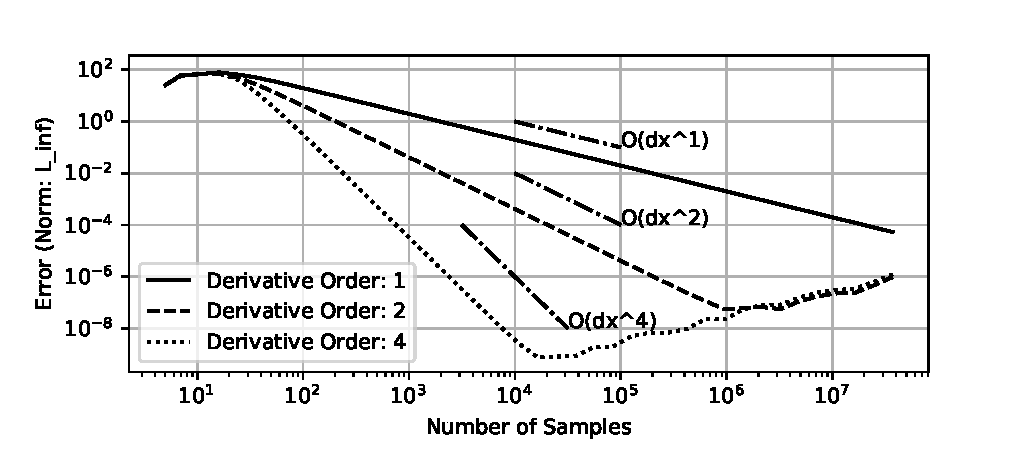
\includegraphics[width=1.2\textwidth]{figures/derivative_error.pdf}}
    \caption{Plot of error of finite difference operators over number of samples}
    \label{fig:derivative_error}
    \small
    The lines are parallel to the expected error order lines, meaning the test was successful.
\end{figure}
It can also be seen that above a certain spacial resolution, the error increases again, which is due to numerical errors.
The root of these errors is the division of a very small number in the denominator by the small number $\Delta x$, which is inversely proportional to the resolution.
This division of small numbers is not well-supported by floating point numbers, and for that reason errors will increase above a certain spacial resolution.\\
Looking at the implementation of the spectral derivative, it is expected that the error will drop down to machine precision as soon as the Nyquist sampling rate is reached.
The Nyquist sampling rate is twice the highest frequency occurring in the signal whose derivative is to be calculated.
In this case the highest frequency is $10$, because the argument of $\sin$ was $2\pi\cdot 10$, meaning the Nyquist sampling rate is $20$.
The fact this theoretical result can be observed in practice (Fig. \ref{fig:fft_error}), is a strong indication that the implementation is correct.

\begin{figure}[!h]
	\makebox[\textwidth]{ 
  		 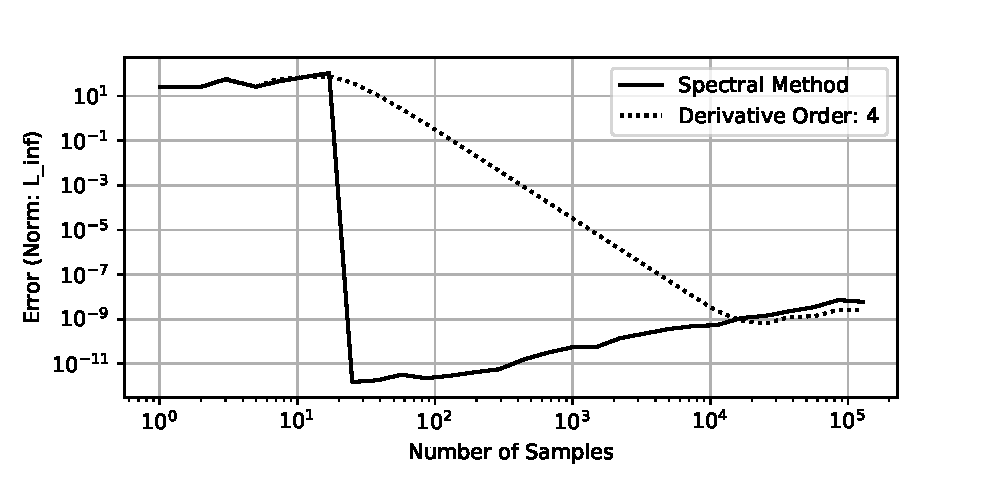
\includegraphics[width=1.2\textwidth]{figures/fft_error.pdf}}
    \caption{Plot of error of spectral derivative operator over number of samples}
    \label{fig:fft_error}
    \small
    As expected the error drops significantly as soon as the Nyquist sampling rate (20 samples) is reached.
\end{figure}

%Test-Function: $\sin(20\pi (x-e))$ on domain $[0;1]$, with resolutions from 5 to $20\cdot 10^7 $
%Actual result is $20\pi\cos(20\pi (x-e))$\\
%show how the error-order is influenced by grid-size.\\
%grid size far larger than features to be measured => inaccuracy\\
%grid size a little bit smaller than features to be measured => change in accuracy according to error-order of implemented operator\\
%grid size too small for machine precision => loss of accuracy

\subsection{Integrators}
\subsubsection{Runge-Kutta-Integrators}
As described in section \ref{sec:testing} the integrators were tested by comparing the results to analytic solution of differential equations.
Specifically, they were first tested against three types of differential equations, whose solutions are known analytically.
The first one was time-invariant and had only one variable, i.e. no spacial resolution.
The second one introduced time-variance into the mix, while the third one added spacial resolution.
In each of the tests, using a Runge-Kutta integrator of order $n$ it was expected that decreasing the time step size by a factor of $a$ would decrease the error by a factor of $a^n$.\\
\paragraph*{Time-Invariant, Single Variable}
The differential equation used is $\frac{dx}{dt}=-3x$, which has the solution $x(t)=x_0e^{-3t}$.
The result of the experiment can be seen in Fig. \ref{fig:RK_error_y'=-3y}.
\begin{figure}[!h]
	\makebox[\textwidth]{ 
  		 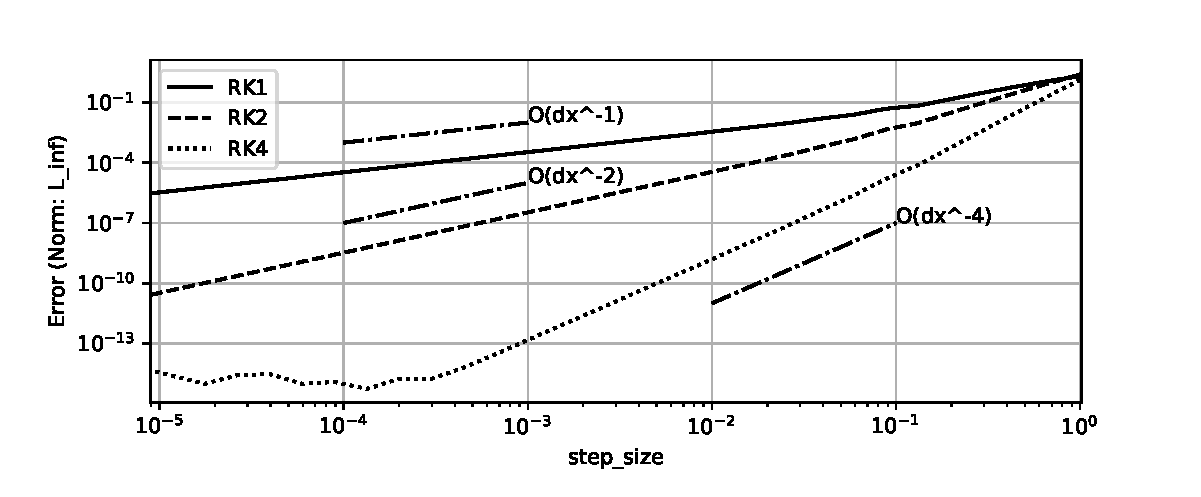
\includegraphics[width=1.2\textwidth]{figures/RK_error_y'=-3y.pdf}}
    \caption{Error of RK-methods on time-invariant, single variable differential equation}
    \label{fig:RK_error_y'=-3y}
\end{figure}

\paragraph*{Time-Variant, Single Variable}
The differential equation used is $\frac{dx}{dt}=\frac{t}{t^2+1}$, which has the solution $x_0 + 0.5\text{ln}(t^2+1)$.
The result of the experiment can be seen in Fig. \ref{fig:RK_error_y'=tdiv(t_t+1)}.
\begin{figure}[!h]
	\makebox[\textwidth]{ 
  		 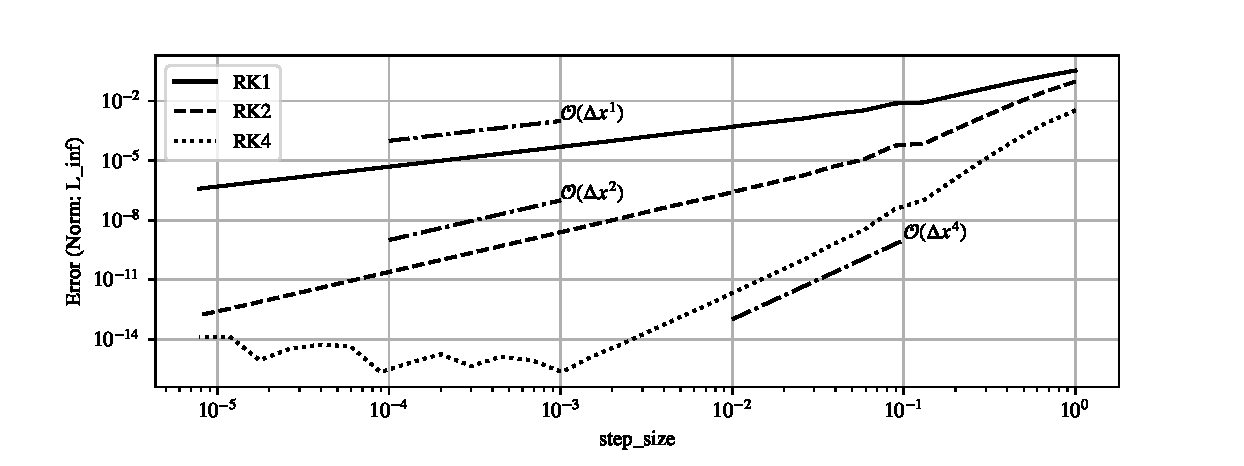
\includegraphics[width=1.2\textwidth]{figures/RK_error_y'=tdiv(t_t+1).pdf}}
    \caption{Error of RK-methods on time-variant, single variable differential equation}
    \label{fig:RK_error_y'=tdiv(t_t+1)}
\end{figure}

\paragraph*{Time-Invariant, Multiple Spatially Distributed Variables}
The differential equation used is the wave equation with periodic boundary conditions.
With $c$ being the wave propagation speed, the equation system can be written as follows:
\begin{align*}
\frac{du}{dt}&=\frac{dv}{dx}\\
\frac{dv}{dt}&=c^2\frac{du}{dx}
\end{align*}
If $u(x,t=0)=f(x)$ (with $f$ being periodic) describes the initial state of $u$, then according to d'Alembert the solution is $u(x,t)=\frac{1}{2}(f(x+ct)+f(x-ct))$, which means $v(x)=\int \frac{du}{dt} dx = \frac{c}{2}(f(x+ct)-f(x-ct))$.

\begin{figure}[!h]
	\makebox[\textwidth]{ 
  		 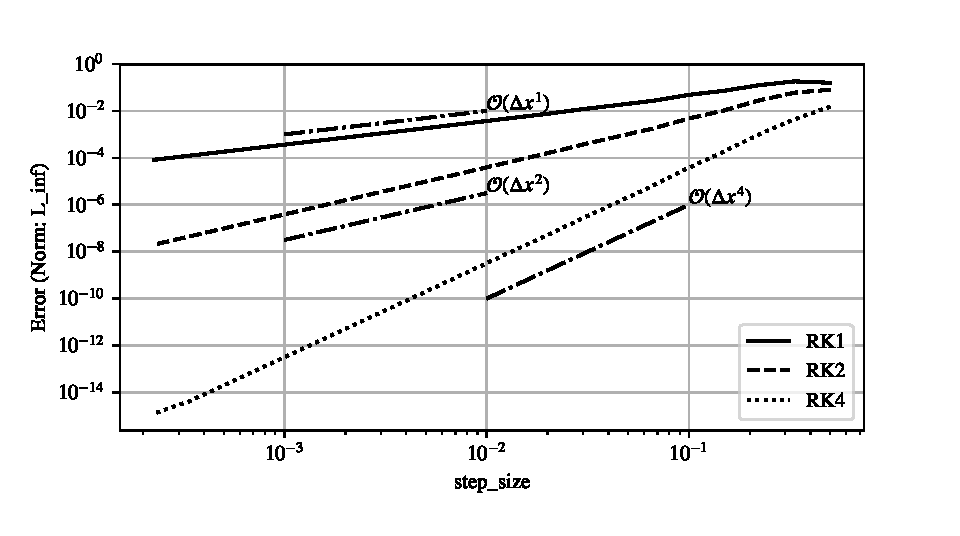
\includegraphics[width=1.2\textwidth]{figures/wave_order_line.pdf}}
    \caption{Error of RK-methods on periodic wave equation}
    \label{fig:wave_order_line}
\end{figure}

Interestingly, spacial resolution and temporal resolution are intertwined, i.e. if a very high spacial resolution (a lot of samples) is chosen, one also has to choose a high temporal resolution (small time steps).
This can be seen when plotting a heatmap of the error made when using the RK4-integrator over different spacial and temporal resolutions.
This phenomenon can be seen in Fig. \ref{fig:heatmap_wave_eq_step_size_numgridpoints}.
Roughly speaking, in order to keep the error from blowing up, an inverse proportion between spacial resolution and time step size should be kept, i.e. when doubling the spacial resolution, one should at least halve the time step size, in order to stay stable.

\begin{figure}[!h]
	\makebox[\textwidth]{ 
  		 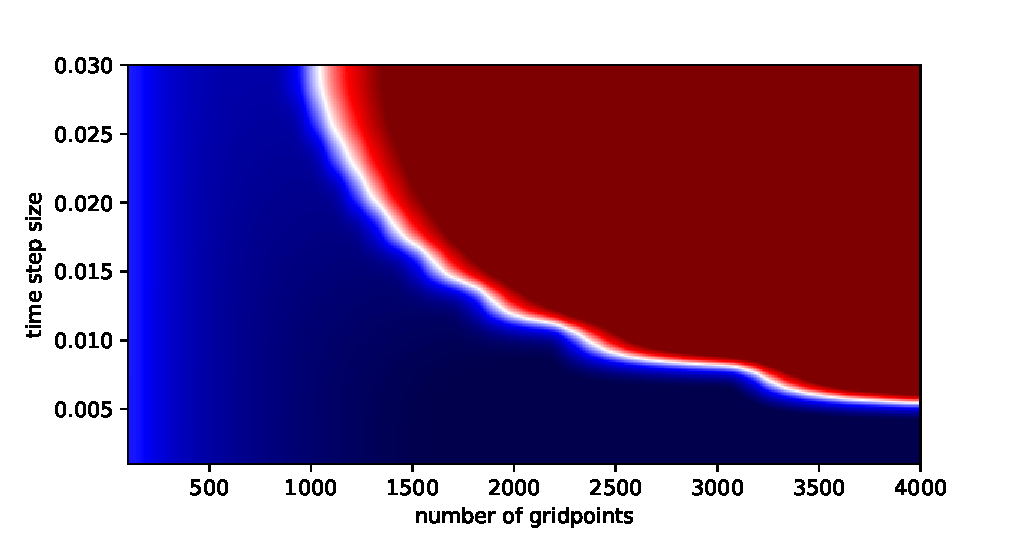
\includegraphics[width=1.2\textwidth]{figures/heatmap_wave_eq_step_size_numgridpoints.pdf}}
    \caption{Heatmap of log(Error) for wave equation over different spacial and temporal resolutions}
    \label{fig:heatmap_wave_eq_step_size_numgridpoints}
	\small
The white stripe represents the area where the log-error is 0, i.e. the actual error is 1.
The red area represents the area where the log-error is positive (can reach values up to $150$), i.e. large.
The blue area represents the area where the log-error is negative (can reach values down to $-20$), i.e. small.
\end{figure}

%$frac{dx}{dt}=\frac{t}{t^2+1}$, which has the solution $x_0 + 0.5\text{ln}(t^2+1)$.



%a time-invariant differential equation with only one variable (i.e. no spacial resolution), then a time-variant differential equation with no spacial resolution, and finally against a differential.
%First off, to verify the implementation, the RK-Integrators were used to solve a differential equation without any spacial resolution, but with temporal variance.
%$\frac{dx}{dt}=\frac{t}{t^2+1}$
%with solution $x_0 + 0.5\text{ln}(t^2+1)$.

%explain how time-step-size and grid-size have to change together, and show trough examples how accuracy changes depending on the choice of these two parameters (maybe a heatmap with x-axis = time-step-size, y-axis=grid-size, color=accuracy after simulation time T?)
%\subsubsection{Exponential Integrators}
%showcase how accuracy stays constant independent of time-step-size (for linear systems)\\
%give a small example of simulating a non-linear system by linearization around the current state


\section{Study of Errors in Implementation of NSE}
In this section the two implementations of the NSE are analyzed.
As no benchmarking systems for testing the vertical of the non-hydrostatic NSE-equations in isolation exist, true verification of the implementation is not possible.
Instead, four tests will be considered:
\begin{itemize}
\item comparison with a stationary solution
\item comparison of stationary solution with real world measurements
\item energy conservation
\item comparison of the two implementations to one another
\end{itemize}
Due to the nature of the non-hydrostatic NSE, mass conservation cannot be used as a test, because mass conservation is always preserved according to equation \ref{eq_mass_conservation}.

\subsection{Comparison with Stationary Solution}
The first way to test the implementations is by verifying that the system state will stay the same, when the starting condition is a stationary solution of the non-hydrostatic NSE.
To find a stationary solution for the non-hydrostatic NSE, all time-derivatives have to be set to zero:
\begin{align}
\frac{\partial w}{\partial t} =0&= -g\left(1 - \frac{\partial p}{\partial s}\left(\frac{\partial \pi}{\partial s}\right)^{-1}\right)\label{stat_dw_dt} \\
\frac{\partial \text{ln}p}{\partial t}=0 &= \frac{g}{1- \frac{R}{C_p}} \frac{p}{RT}\left(\frac{\partial \pi}{\partial s}\right)^{-1} \frac{\partial w}{\partial s}\label{stat_dlnp_dt}\\
\frac{\partial T}{\partial t} =0&= \frac{RT}{C_p}\frac{\partial \text{ln}p}{\partial t}\label{stat_dT_dt}
\end{align}
The first equation \ref{stat_dw_dt} yields the following identity for pressure:
\begin{align*}
\frac{\partial p}{\partial s}=\left(\frac{\partial \pi}{\partial s}\right)\\
\Rightarrow p(s)=\pi (s) + p_0
\end{align*}
The second equation \ref{stat_dlnp_dt} is requires one of the elements in the denominator to equal zero.
As neither $g$, $p$, nor $\left(\frac{\partial \pi}{\partial s}\right)^{-1}$ can be zero, the only possible option is that $\frac{\partial w}{\partial s}=0$, i.e. $w(s)=w_0 \forall s$.
Due to the boundary conditions, at the bottom of the atmosphere $w(1)=0$, so $w(s)=w_0 \forall s$.\\
The last equation \ref{stat_dT_dt} yields no information, because the right hand side is already zero, due to $\frac{\partial \text{ln}p}{\partial t}=0$.
This means $T$ can be chosen freely, e.g. $T=273K$.\\
Using this stationary solution to define the initial state of the system, the integrator is expected not to change the system state.
This is reflected by both implementations as can be seen in Fig. \ref{fig:lorenz_stat_err}, where the magnitude of the error is never greater than $10^{-8}$.

\begin{figure}[!h]
	\makebox[\textwidth]{ 
  		 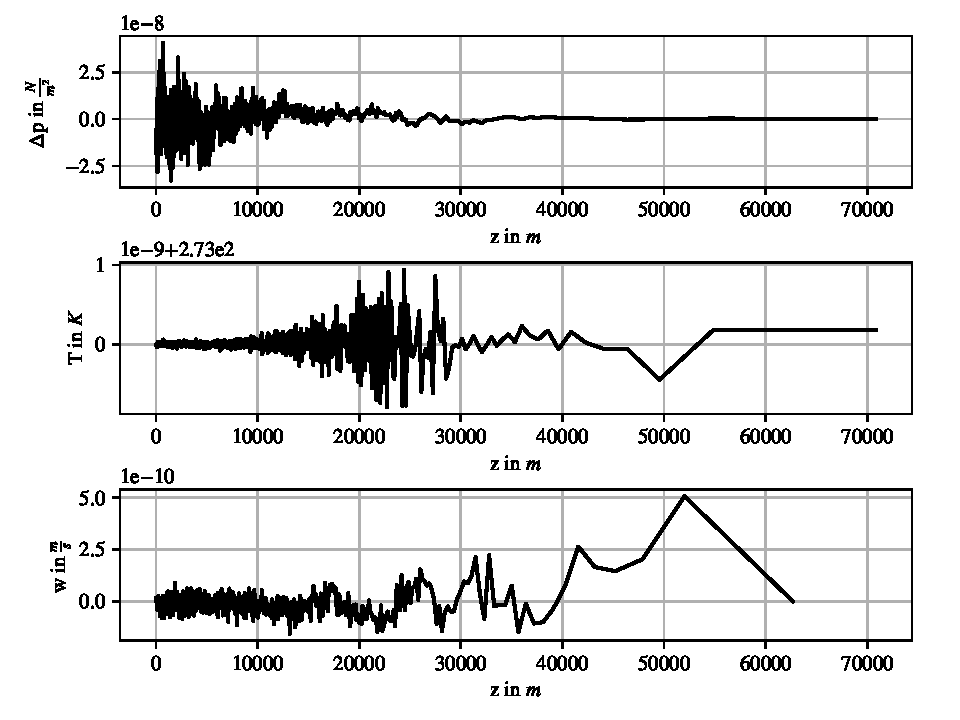
\includegraphics[width=1.2\textwidth]{figures/lorenz_240s_stat.pdf}}
    \caption{Error (deviation from stationary solution) made using RK4, time-step-size $2.5ms$, and $1000$ grid points, after $240s$ of simulation time on Lorenz grid (the corresponding diagram \ref{fig:cp_stat_err} for the Charney-Phillips-grid is nearly identical and can be found in the appendix)}
    \label{fig:lorenz_stat_err}
\end{figure}

\subsection{Comparison with Real World Measurements}
Another method to test the implementation is to compare measurements from the real world with measurements made within the implementation.
First, one can compare the distribution of density $\rho=\frac{p}{RT}$ in the stationary case to real world measurements made by NASA \cite{larson1963stratosphere} of the atmosphere.
For the simulation it was assumed that pressure at the bottom of the system was $\pi_{bottom}=1atm=101325 Pa$, and $T=273K$.
Also it was assumed that $\pi (s) = s\cdot\pi_{bottom}$
In Fig. \ref{fig:cmp_nasa} it can be seen that the calculated result closely mirrors reality.


\begin{figure}[!h]
	\makebox[\textwidth]{ 
  		 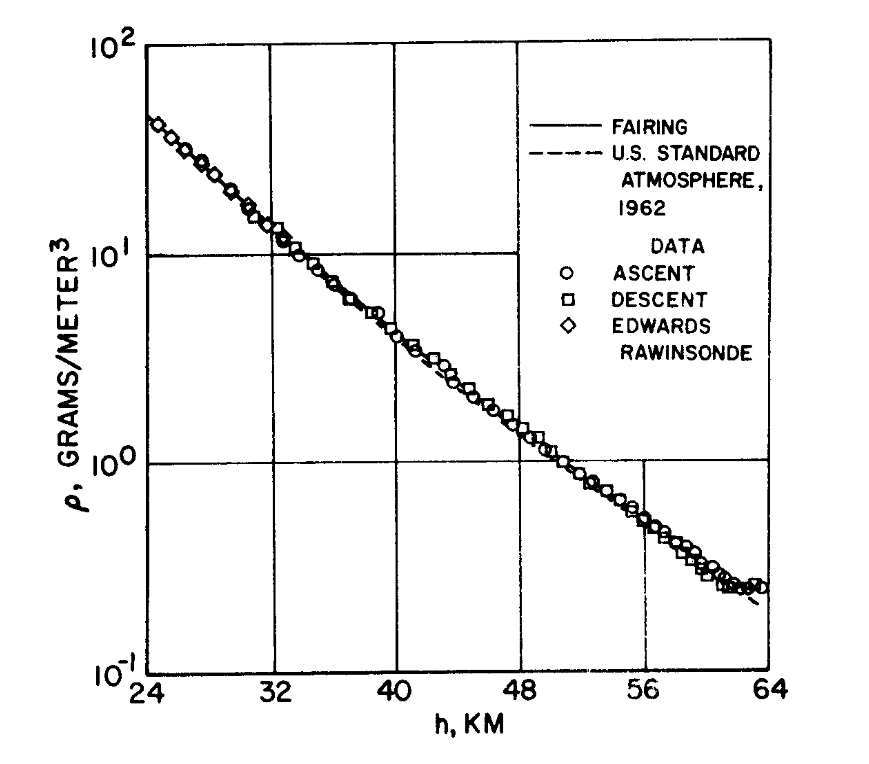
\includegraphics[width=0.5\textwidth]{figures/height_density_nasa.png}
  		 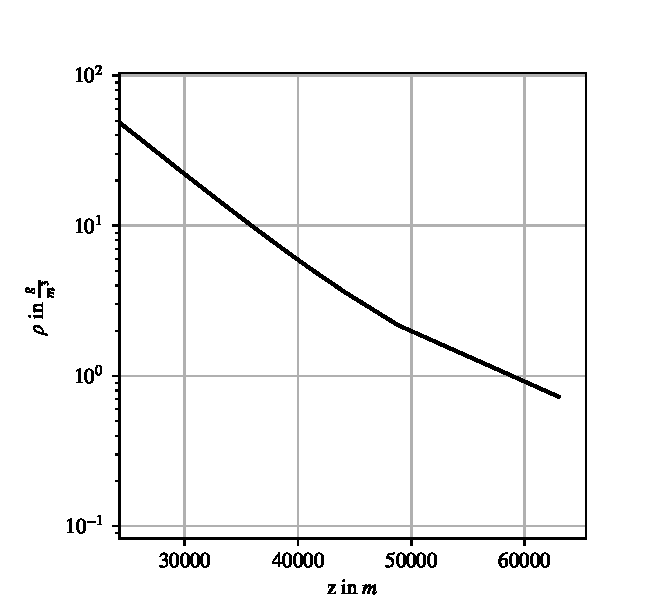
\includegraphics[width=0.5\textwidth]{figures/height_density.pdf}}
    \caption{Comparison of real world measurements from NASA \cite{larson1963stratosphere} with simulated results.}
    \label{fig:cmp_nasa}
\end{figure}

The second comparison with real world measurements is the speed of sound.
The speed of sound is essentially nothing but the speed at which a region of increased pressure will travel.
In other words the wave speed of the system.
To measure wave speed, first, an appropriate starting condition containing a region of increased pressure has to defined, and then the location of this bump has to measured over time.
From the trace of time and location, speed can be calculated through the derivative.\\
The result of such an experiment can be seen in Fig. \ref{fig:sound_speed}, namely that the speed of sound in the simulation ranges between $331\frac{m}{s}$ and $341\frac{m}{s}$.
This is close to the actual speed of sound at sea level around $331\frac{m}{s}$ according to \cite{hardy1942velocity}.

\begin{figure}[!h]
	\makebox[\textwidth]{ 
  		 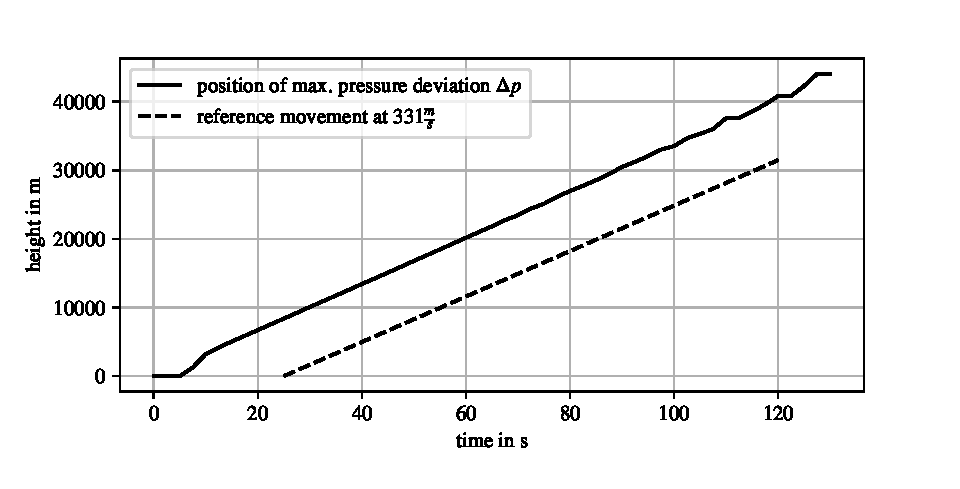
\includegraphics[width=1.0\textwidth]{figures/sound_speed.pdf}}
    \caption{Graph of location over time of (a) a region of increased pressure; (b) a reference object moving at the speed of sound ($331\frac{m}{s}$)}
    \label{fig:sound_speed}
    \small
    The simulation was run using $1000$ grid points and a time step size of $2.5ms$ on a Lorenz-grid. Simulations using Charney-Phillips-grids yield similar results.
\end{figure}

For the experiment, the starting condition was chosen as follows: $T=273K$, $w=0$.
For $p$, first, the stationary solution was used as a baseline, i.e. $p(s)=\pi (s)$.
Then a Gaussian bellcurve of magnitude $1\frac{N}{m^2}$ with its maximum at the bottom $s=1$ was added onto this configuration.
Inserting the Gaussian bump at any other location but the boundary of the domain would result in two regions of increased pressure traveling across the atmosphere, which would make the measurement more difficult.\\
Note that this is one of the key differences between simulation using the hydrostatic NSE versus using the non-hydrostatic NSE.
According to Coiffier, using the hydrostatic NSE "eliminates sound waves because of the nydrostatic relation which has a \emph{filtering} effect on them"\cite{coiffier2011fundamentals}.

\subsection{Energy Conservation}\label{sec:energy_conservation_test}
The third way of testing the implementation is by testing the hypothesis of energy conservation.
As the choice of boundary conditions dictates that energy in the system must stay constant, every simulation of the non-hydrostatic NSE should have the same property.
That is, every system state produced by the simulation should have the same energy as the starting condition.\\
To this end the formula for calculating the total energy in the system per area \ref{eq_energy} is used.
\begin{align*}
E'=\int_{s_{top}}^{s_{bottom}} \frac{1}{g}(C_vT+\frac{1}{2}w^2 + gz(s)) \left( \frac{\partial \pi}{\partial s} \right) ds
\end{align*}
When assuming energy to stay constant over time, it makes sense to use the energy contained in the system at the beginning as a baseline.
This way, by subtracting the baseline energy from the energy calculated at some later time during simulation, the error can be tracked over time.\\
Of course, in order for it to be possible for an error to appear, the system must change over time, i.e. not be stationary.
Other than that any starting condition may be chosen.
For the following simulations, the starting conditions were as follows: $T=273K$, $w=0$.
For $p$, first, the stationary solution was used as a baseline, i.e. $p(s)=\pi (s)=s\cdot 101325\frac{N}{m^2}$.
Then a Gaussian bellcurve of magnitude $0.1\frac{N}{m^2}$ with its maximum at $z=35km$ was added onto this configuration.
\\
The results of this for both the Lorenz-grid and the Charney-Phillips-grid can be seen in Fig. \ref{energy_error}.
The baseline energy for both was $3163398684.51234J$.

\begin{figure}[!h]
	\makebox[\textwidth]{ 
  		 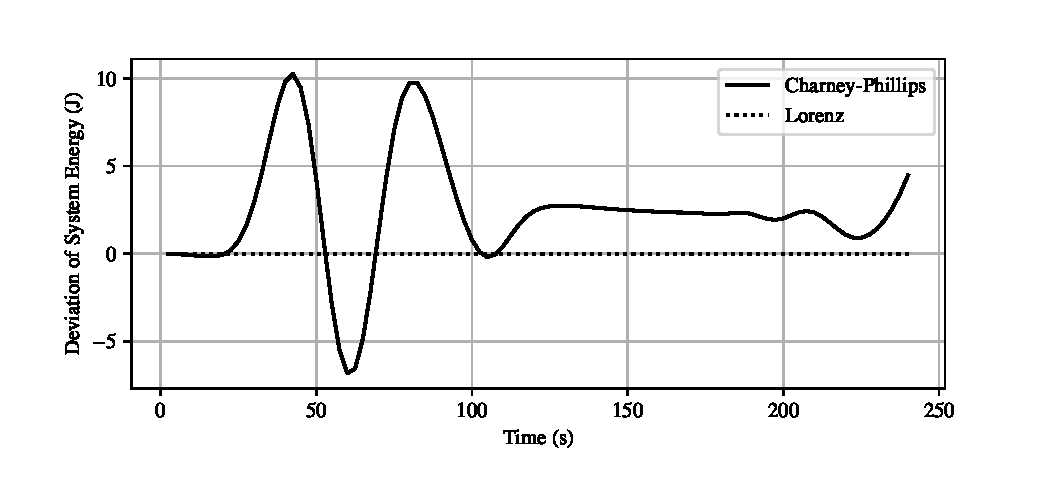
\includegraphics[width=1.0\textwidth]{figures/cp_energy_error.pdf}}
  	\makebox[\textwidth]{
  		 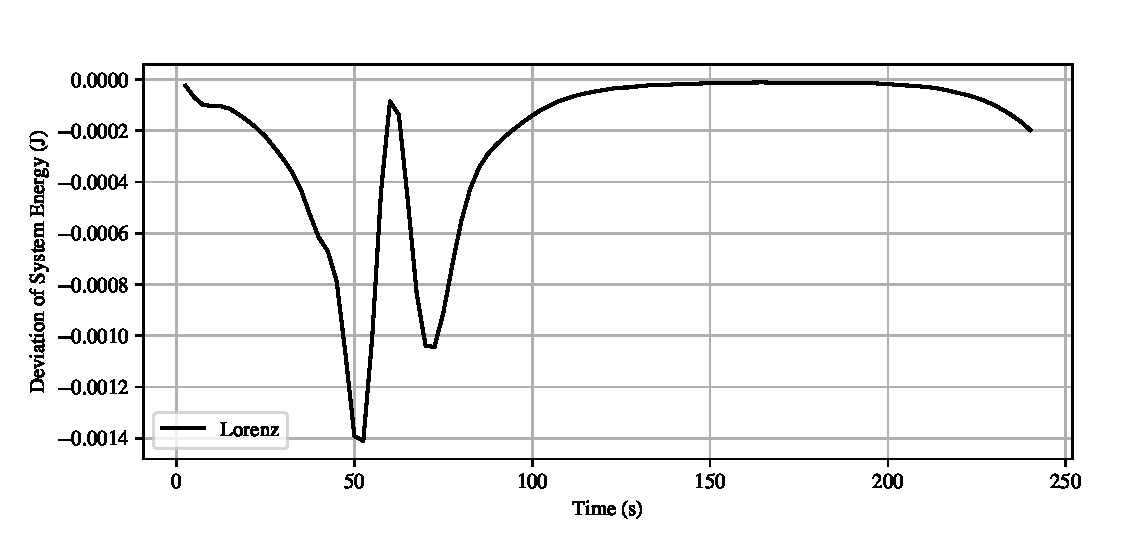
\includegraphics[width=1.0\textwidth]{figures/lorenz_energy_error.pdf}}
    \caption{Energy deviation over time for Lorenz-Grid and Charney-Phillips-grid.}
    \label{fig:energy_error}
    \small
Both simulations were run using $1000$ grid points and a time step size of $2.5ms$.
\end{figure}

To explain the larger error when using the Charney-Phillips-grid, one has to look at the composition of energy.
Recall that energy in the atmospheric system can be split up into three components: internal energy, kinetic energy, and geopotential energy.

\begin{figure}[!h]
	\makebox[\textwidth]{ 
  		 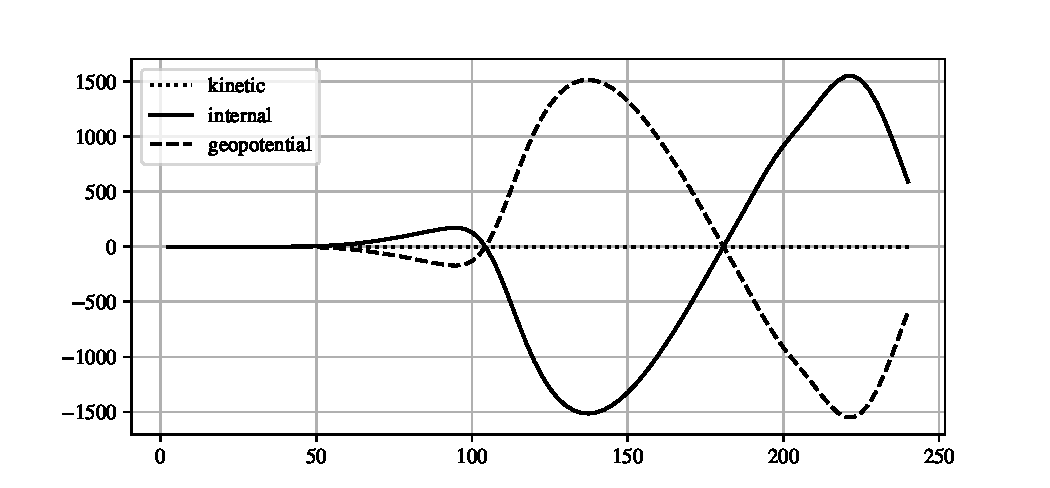
\includegraphics[width=1.0\textwidth]{figures/cp_energy_split.pdf}}
    \caption{Deviation of each component of energy over time for Charney-Phillips-grid.}
    \label{fig:cp_energy_split}
    \small
    The simulation was run using $1000$ grid points and a time step size of $2.5ms$.
\end{figure}

When plotting the individual deviations for each component, as is done in Fig. \ref{fig:cp_energy_split}, one can see that the kinetic energy deviation is almost negligible at around $3\cdot10^{-3}J$.
Instead the discrepancy for the Charney-Phillips-grid must originate from an asymmetry between the deviation of internal and geopotential energy.
While not certain, this asymmetry is probably rooted in the manner the time-derivative for temperature $T$ is calculated numerically.\\
Recall the prognostic equation for $T$:
\begin{align*}
\frac{\partial T}{\partial t} &= \frac{RT}{C_p}\frac{\partial \text{ln}p}{\partial t}\\
&=\frac{gp}{C_p-R}\left(\frac{\partial \pi}{\partial s}\right)^{-1} \frac{\partial w}{\partial s}
\end{align*}
It can be seen that $T$ either depends on $\frac{\partial \text{ln}p}{\partial t}$, or $p$ (when substituting in the prognostic equation for $\frac{\partial \text{ln}p}{\partial t}$).
For the Charney-Phillips-grid, both of these variables are sampled on the offset grid, meaning that in order to calculate $\frac{\partial T}{\partial t}$, an averaging operator has to be applied, which is not especially accurate.\\
In light of this, the Lorenz grid should be preferred when simulating the non-hydrostatic NSE.

\subsection{Comparison of the two Implementations}
The final way the two implementations were tested, is by comparing the simulation outputs, after a certain amount of elapsed time.
For purposes of this test, both implementations were initialized with identical starting conditions.
Just like in the previous section, any starting condition can be chosen.
For simplicity's sake, the same starting condition as in the previous section \ref{sec:energy_conservation_test} was used.\\
Using said starting condition, both simulations were run for $240s$ of simulation time, using a spacial resolution of $1000$ grid points, and a temporal resolution of $2.5ms$.
The result of the two simulations on the different grids can be seen in Fig. \ref{fig:simulations}.\\
The similar look of the separate simulation results for pressure deviation $\Delta p$ and vertical wind speed $w$ is no optical illusion.
It can also be verified numerically:
When taking the difference between the two simulation results, the largest absolute difference\footnote{Also known as the $L_\infty$-norm} for $\Delta p$ is $8.71\cdot 10^{-11}$, and the largest absolute difference for $w$ is $9.32\cdot 10^{-9}$.
The difference for $T$ was not determined, because the two $T$-grids are offset to one another by definition of the Charney-Phillips and Lorenz grids, so any comparison would have taken place through inaccurate averaging operations.\\
The minuscule difference of $\Delta p$ and $w$ between implementations reaffirms the assumption made in section \ref{sec:energy_conservation_test} that the error in energy conservation for the Charney-Phillips grid must stem from inaccuracies in $T$.

\begin{figure}[!h]
	\makebox[\textwidth]{ 
  		 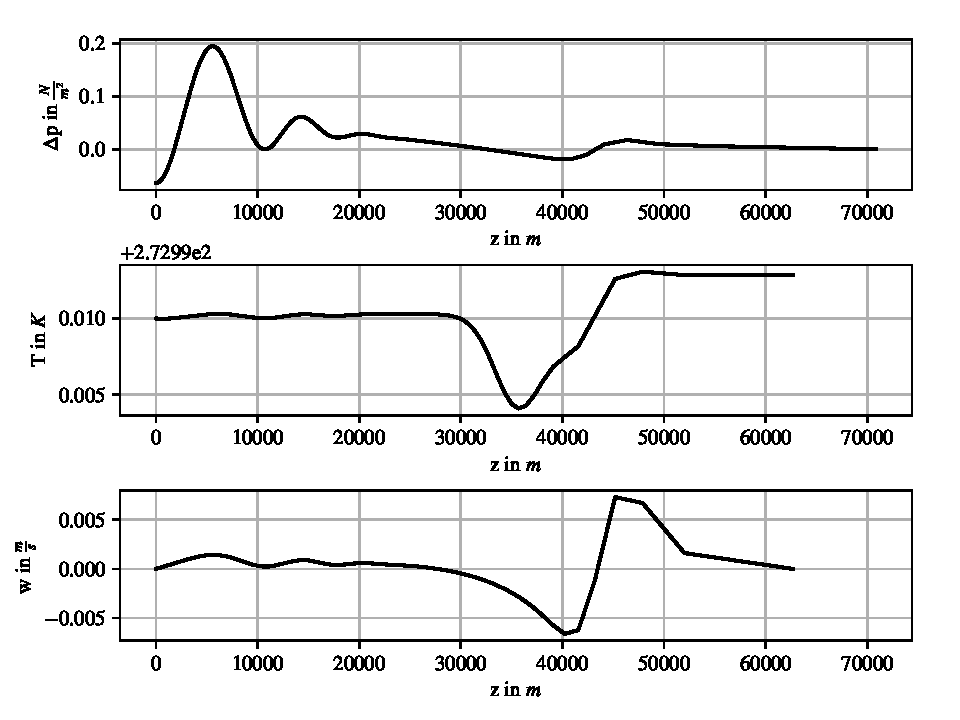
\includegraphics[width=0.8\textwidth]{figures/cp_240s_bump.pdf}}
  	\makebox[\textwidth]{
  		 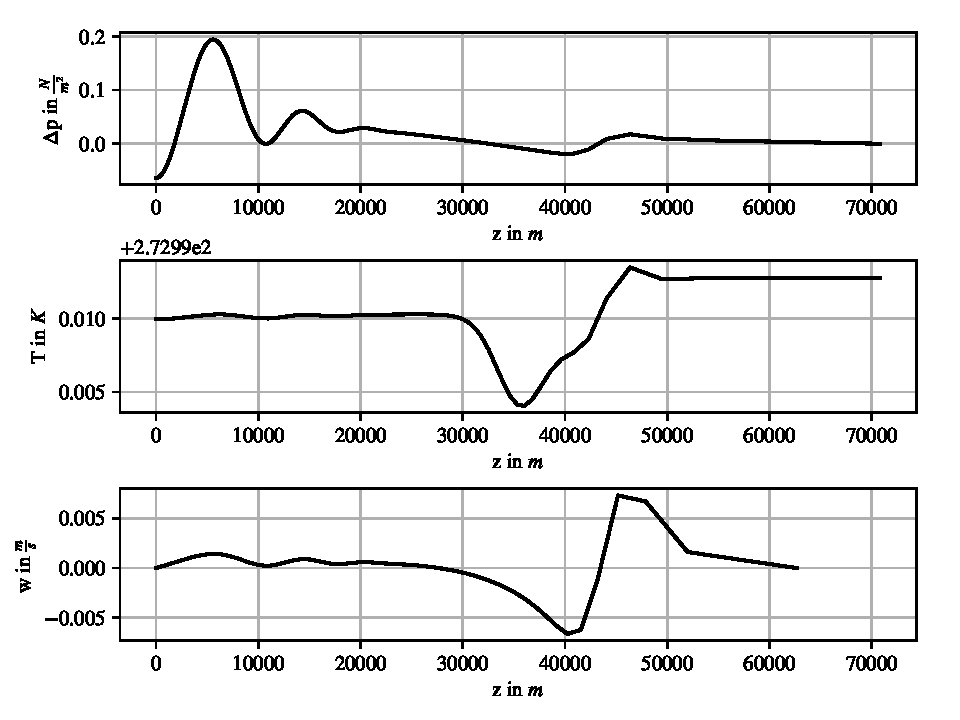
\includegraphics[width=0.8\textwidth]{figures/lorenz_240s_bump.pdf}}
    \caption{Simulation results using the Charney-Phillips grid (first three diagrams), and the Lorenz grid (last three diagrams).}
    \label{fig:simulations}
    \small
Both simulations were run using $1000$ grid points and a time step size of $2.5ms$.
\end{figure}


In summary, both implementations pass all tests

%In this section the effects (all?) possible choices of simplifications, integrators etc. is analyzed.\\
%To this end we introduce different ways of measuring errors, i.e. different norms, and use them to measure the difference between different simulations.

%\subsection{Simplifications to the Navier Stokes Equations} % effects of simplifications
%have one simulation without simplifications run with high precision (RK4 with tiny step-sizes and high grid resolution), and compare that to simulations using high precision with simplifications.

%\subsection{Grid Discretizations}% grid discretizations
%Quantify the difference between the two different grids.
%How do we really know which one is better?
%Find ways to quantify which one is more accurate?